
% https://github.com/xinychen/awesome-latex-drawing
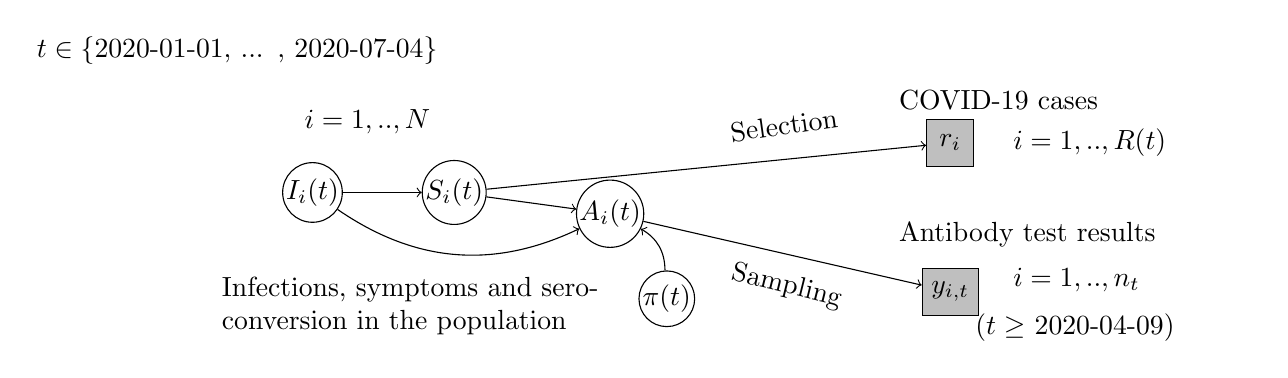
\begin{tikzpicture}[
    scale = 0.9,
    param/.style={shape=circle, draw=black,fill=white,inner sep=0pt,minimum size=0.6cm},
    obs/.style={shape=rectangle, draw=black, fill=lightgray, minimum size=0.6cm}
  ]
  
    % time t
    \node [text width=7cm] (T) at (-3.0, 1)  {$t \in \{$\printdate{2020-01-01}, ... , \printdate{2020-07-04}$\}$};
    
    % infections
    \node [param] (inf) at (-3,-1) {$I_i(t)$};
    
    % symptoms
    \node [param] (symp) at (-1,-1) {$S_i(t)$};    
    
    % antibodies
    \node [param] (sero) at (1.2,-1.3) {$A_{i}(t)$};
    
    % seroprevalence
    \node [param] (prevalence) at (2, -2.5) {$\pi(t)$};
    
    
    % text for population plate
    \node [text width=5cm] (latent) at (-1.5,-2.6)  {Infections, symptoms and seroconversion in the population};
    
    % label and plate for population
    \node [text width=2cm] (N) at (-2, 0)  {$i = 1, .., N$};
    \plate[]{POP}{(inf)(sero)(N)(latent)(prevalence)}{};

    
    % registered disease cases
    % ---
    
    % Selection
    \node [text width=2cm, rotate=8] (ttrsampling) at (4,0) {Selection};
    
    % r_i
    \node [obs]  (ttr) at (6,-0.3) {$r_i$}; 
    
    % label
    \node [text width=4cm] (registry) at (7.5,0.3) {COVID-19 cases};
    
    % R(t)
    \node [text width=2cm] (nobs) at (8,-0.3)   {$i = 1, .., R(t)$};  
    

    
    % Antibody test results 
    % ---
    
    % Sampling
    \node [text width=2cm, rotate=-14] (serosampling) at (4, -1.5*1.6) {Sampling};    
    
    %  y
    \node [obs]  (y) at (6,-1.5*1.6) {$y_{i, t}$};   
    
    % label
    \node [text width=4cm] (serosurvey) at (7.5,-1.6)  {Antibody test results};

    % n_t
    \node [text width=2cm] (nsero) at (8,-1.6*1.4)  {$i = 1, .., n_{t}$};  
    
    % t sero
    \node [text width=3.5cm] (serosurvey_t) at (8.3,-2.9)  {($t \geq$ \printdate{2020-04-09})};


    
    % paths
    \path [draw,->] (inf) edge (symp);
    \path [draw,->] (inf) edge [bend right] (sero);
    \path [draw,->] (symp) edge (sero);
    \path [draw,->] (sero) edge (y);
    \path [draw,->] (symp) edge (ttr);
    
    \path [draw,->] (prevalence) edge [bend right] (sero);

    % plate for antibody observations
    \plate[]{SERO}{(y)(serosurvey)(nsero)}{}
    
    % plate for infection observations
    \plate[]{TTR}{(ttr)(registry)(nobs)}{}
    
    
    \plate[]{TIME}{(T)(POP)(TTR)(SERO)}{}
    
    \plate[white]{ALL}{(TIME)}{}
    
 
    
\end{tikzpicture}